\chapter{DATASET, DATABASE AND DESIGN OF THE NDVI APPLICATION}
\label{chap:dataset & database}

\section{NDVI dataset and its significance}

\subsection{About MODIS}

\newcommand{\MYhref}[3][blue]{\href{#2}{\color{#1}{#3}}}%

\centerline{\MYhref{https://modis.gsfc.nasa.gov/}{NASA's MODIS website}}

\gls{modis} is a key instrument on board the Terra (initially known as EOS AM-1) and Aqua (initially known as EOS PM-1) satellites. Land's circle around the Earth is coordinated with the goal that it goes from north to south over the equator early in the day, while Aqua disregards south to north the equator toward the evening. Land \gls{modis} and Aqua \gls{modis} are seeing the whole Earth's surface each 1 to 2 days, gaining information in 36 ghastly groups, or gatherings of wavelengths (see \gls{modis} Technical Specifications). These information will enhance our comprehension of worldwide elements and procedures happening on the land, in the seas, and in the lower climate. \gls{modis} is assuming a fundamental job in the improvement of approved, worldwide, intuitive Earth framework models ready to foresee worldwide change precisely enough to help arrangement creators in settling on quality choices concerning the security of our condition. \cite{MODIS} \\

\centerline{\textbf{Terra vs. Aqua}}

According to \gls{nsidc} distributes \gls{modis} data from both the Terra and Aqua satellites.

Figure 3.1 shows the difference between the two satellites. For the application, we have worked with Aqua satellite's data.

 \begin{figure}[H]
            \centering
            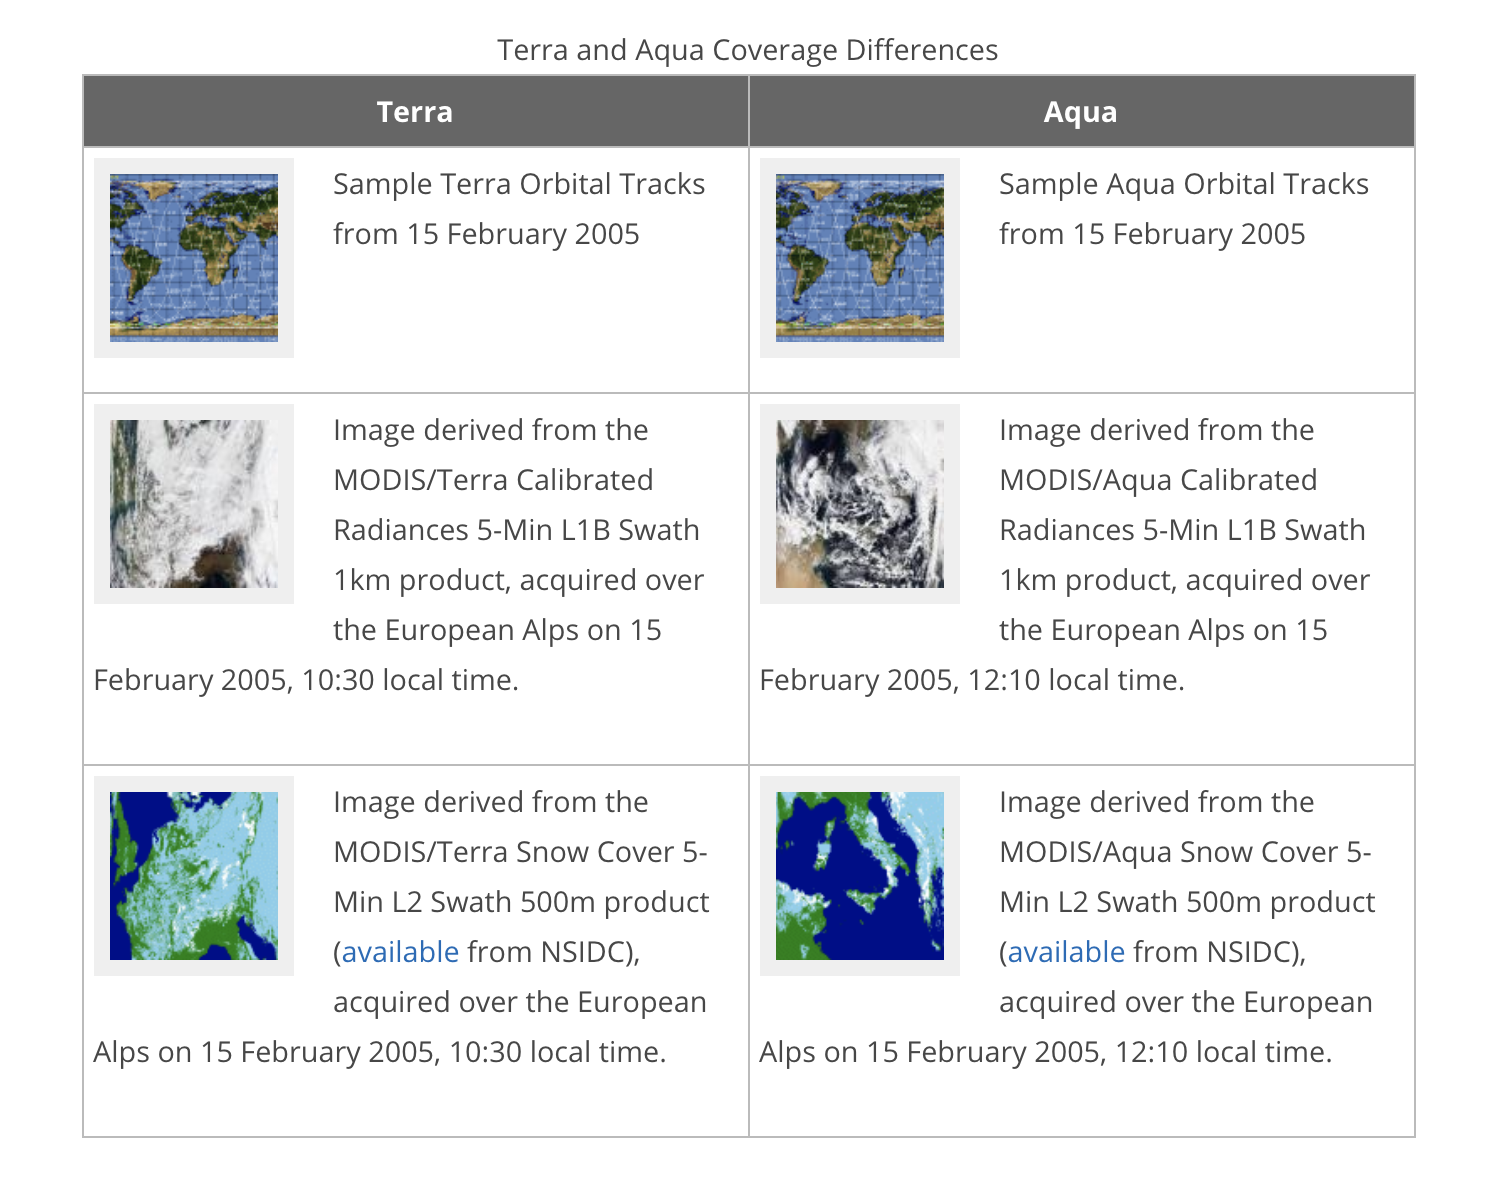
\includegraphics[width=1.0\linewidth]{figures/ch3/satellites.png}
            \caption{\label{fig:modis_satellites_difference} Difference between MODIS satellites \cite{NSIDC}}
    \end{figure}

\subsection{Overview of NDVI Dataset}

\gls{modis} vegetation indices, delivered on 16-day interims and at various spatial goals, give steady spatial and worldly correlations of vegetation covering greenness, a composite property of leaf territory, chlorophyll and shade structure. Two vegetation lists are gotten from environmentally redressed reflectance in the red, close infrared, and blue wavebands; the standardized contrast vegetation list \gls{ndvi}, which gives coherence \gls{noaa}'s AVHRR \gls{ndvi} time arrangement record for verifiable and atmosphere applications, and the upgraded vegetation list (EVI), which limits covering soil varieties and enhances affectability over thick vegetation conditions. The two items all the more successfully describe the worldwide scope of vegetation states and procedures. 

As of now, NASA has the website to utilize the GIMMS Global Agricultural Monitoring (GLAM) System to see MODIS NDVI symbolism and recover MODIS NDVI time arrangement information. The framework gives close ongoing and science quality Terra and Aqua MODIS 8-day composited, worldwide NDVI datasets. These datasets are gotten from the Collection 6 MOD09 and MYD09 surface reflectance items which are given by NASA/GSFC/EOSDIS LANCE and NASA/GSFC MODAPS.

The GIMMS MODIS GLAM System is produced and given by the NASA/GSFC/GIMMS bunch for the USDA/FAS/IPAD Global Agricultural Monitoring venture. The USDA/FAS/IPAD mission is to give objective, auspicious, and consistent appraisal of the worldwide agrarian generation standpoint and conditions influencing worldwide sustenance security.

Please see the figures 3.2 and 3.3 for user guide of the website.

    \begin{figure}[H]
            \centering
            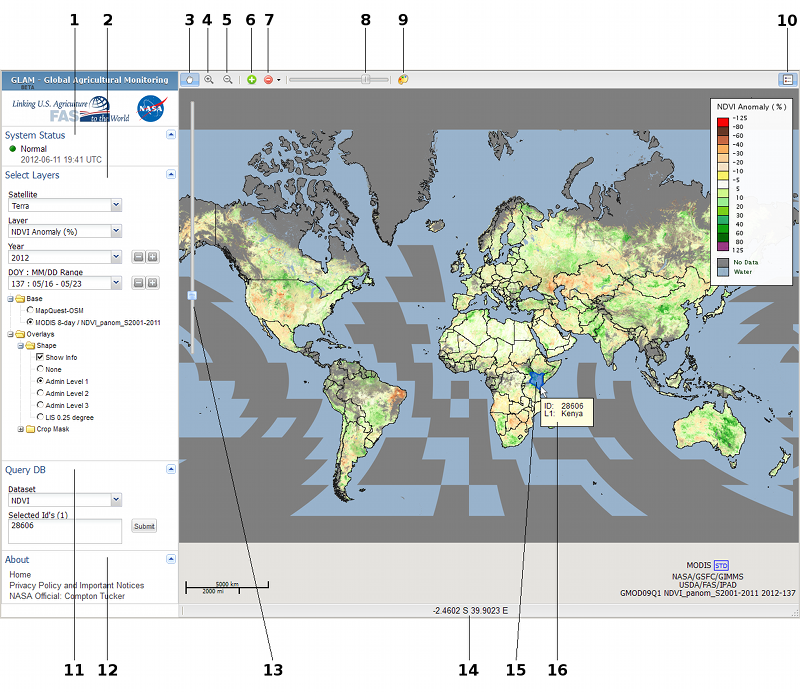
\includegraphics[width=1.0\linewidth]{figures/ch3/nasa_website_1.png}
            \caption{\label{fig:nasa_website_1} NASA's NDVI website user guide part-I \cite{GAM}}
    \end{figure}
    
    
    \begin{figure}[H]
            \centering
            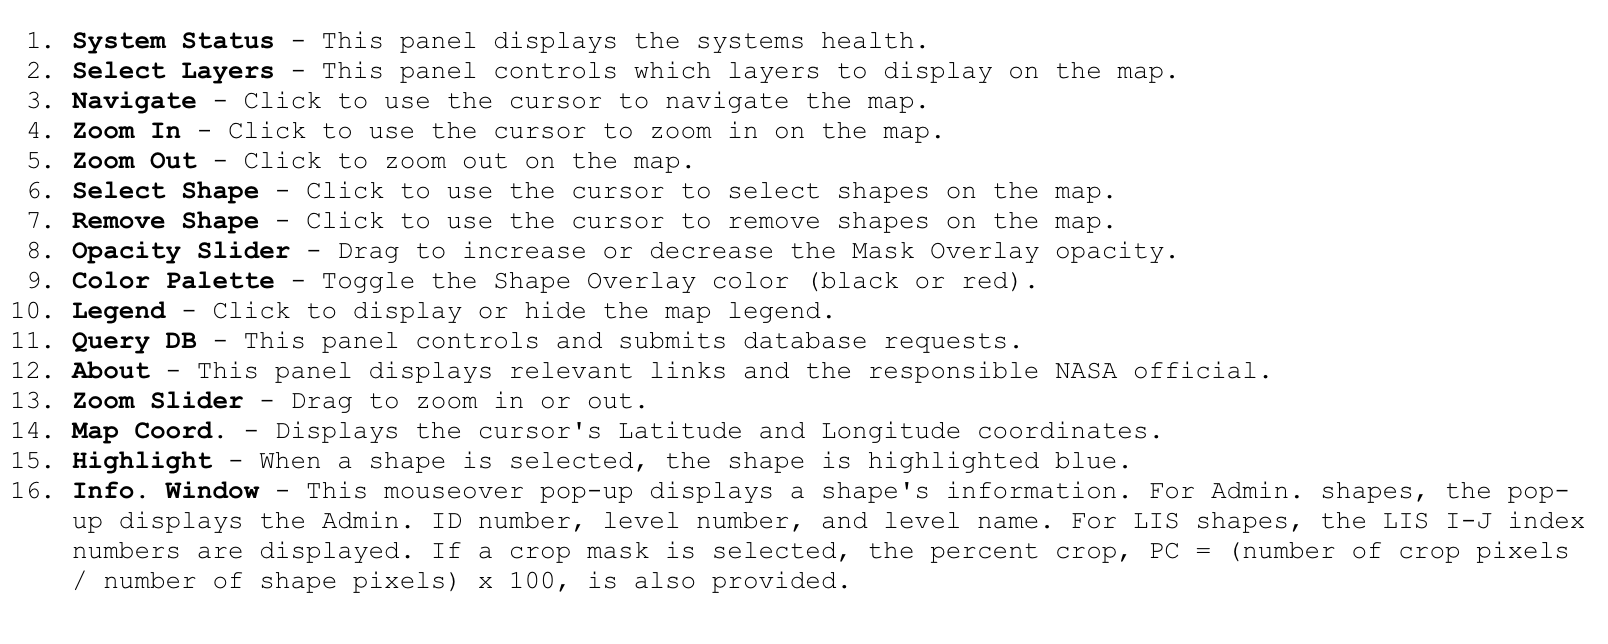
\includegraphics[width=1.0\linewidth]{figures/ch3/nasa_website_2.png}
            \caption{\label{fig:nasa_website_2} NASA's NDVI website user guide part-II \cite{GAM}}
    \end{figure}    


The vegetation records are recovered from day by day, air redressed, bidirectional surface reflectance. The VI's utilization a \gls{modis}-particular compositing strategy dependent on item quality confirmation measurements to evacuate low quality pixels. From the staying great quality VI esteems, an obliged see edge approach at that point chooses a pixel to speak to the compositing time frame (from the two most elevated \gls{ndvi} esteems it chooses the pixel that is nearest to-nadir). Since the \gls{modis} sensors on board Terra and Aqua satellites are indistinguishable, the VI calculation creates every 16-day composite eight days separated (staged items) to allow a higher worldly goals item by joining the two information records. The \gls{modis} VI item suite is currently utilized effectively in all environment, atmosphere, and regular assets administration contemplates and operational research as exhibited by the consistently expanding group of associate distributions. \\

\centerline{\textbf{How do you calculate NDVI?  \cite{theGISGeography}}}

\textbf{\[ NDVI = \frac{NIR - RED}{NIR + RED} \ \ \ 
\ \ \]}

\centerline{NIR: \gls{nir}}
\centerline{RED: \gls{red}}

Solid vegetation (chlorophyll) reflects more close \gls{nir} and green light contrasted with different wavelengths. In any case, it retains more red and blue light. 

This is the reason our eyes consider vegetation to be the shading green.

Let's look at the example shown in the fig 3.4.

    \begin{figure}[H]
            \centering
            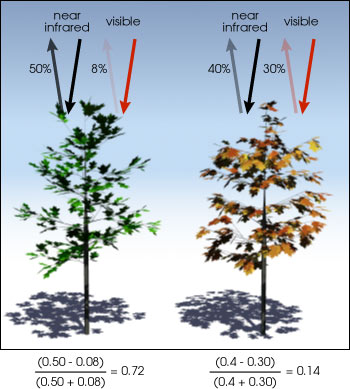
\includegraphics[width=0.5\linewidth]{figures/ch3/ndvi-example.png}
            \caption{\label{fig:ndvi_example} NDVI Example - Courtsey: NASA \cite{MODIS}}
    \end{figure}

Data is normally stored in a \gls{gdac} \gls{ftp} server, at a US-based server at \url{https://gimms.gsfc.nasa.gov/MODIS/}.

The information is thought to be adequately quality controlled and in a steady arrangement. Stage and profile name is the main distinguishing proof. This information structure does not permit regular determination or spatial choice: a key element to any atmosphere informational index. The FTP server is intended to go about as a chronicle. Researchers are urged to download the information locally for their utilization's, a procedure that depends on noteworthy space learning of the FTP website. Barely any individuals will experience the inconvenience of understanding the FTP structure, less still will set aside opportunity to make the procedure less demanding for other people.

\subsection{Significance}

The term \gls{ndvi} in the farming business has positively increased more mindfulness of late because of the developing ubiquity of little unmanned elevated vehicles. 

\gls{ndvi} is positively not another child on the square and with regards to social affair and preparing this data, rural experts have known and been utilizing this information for quite a long time. Anyway already assembling this information may have been tedious, awkward, not exceptionally precise and costly. 

As innovation enhances and the methods in which we would now be able to catch this information, agriculturists are beginning to take this basic and successful information all the more genuinely by hoping to join this technique into their product administration methodology. 

Information is enter in exactness farming, knowing your product's well being is a certain something yet really pre-empting the state of harvest's well being, endorsing compost application, distinguish any potential sickness and precisely assessing yield puts the control in your grasp consequently making you all around educated to settle on the correct business choices as and when required.

\gls{ndvi} is valuable for evaluating the well being and thickness of vegetation. \gls{ndvi} esteems close to 0 show extremely inadequate vegetation. Thick vegetation is demonstrated by \gls{ndvi} esteems moving toward 1. By utilizing a period arrangement of \gls{ndvi} perceptions, one can look at the elements of the developing season and screen wonders, for example, dry spell. A full supplement of information has been finished from the earliest starting point of Terra satellite activity to the present and is accessible for download in peruse and 250m goals.


\section{Wireframes Designs}

A versatile application wireframe, otherwise called a page schematic or screen outline, is a visual guide that speaks to the skeletal structure of an application. Wireframes are made to arrange components to best achieve a specific reason.

In other words, they are the skeleton of any product. This skeleton is a two-dimensional delineation of a page's interface that demonstrates the dividing of components on the page, how content is organized, what functionalities are accessible, and how clients will cooperate with the site. They likewise assume an essential job in interfacing data engineering to the visual parts of the outline by indicating pathways between the different pages. Wireframes are purposefully drained of shading, illustrations and adapted textual styles. The tool used for creating wireframes here is \textbf{Axure RP 8}. \\

Reasons for using wireframes are mentioned below:

\begin{itemize}
    \item Wireframes enable you to outline the usefulness of the pages, get issues early, and spare time on corrections later. It is considerably less excruciating to roll out improvements to a wireframe than to a high devotion mockup with heaps of plan components. \\
    
    \item Wireframes are an incredible method to organize content by uncovering space requirements and planning the pecking order of components on the page. Having the open door right off the bat to envision the chain of command of your pages and start outwardly showing the space requirements will spare you a ton of time later when you start adapting the pages and filling them with substance. \\
\end{itemize}

\centerline{\textbf{Some of the Wireframes designs are shown below in figure 3.5, 3.6 and 3.7}} 

    \begin{figure}[H]
            \centering
            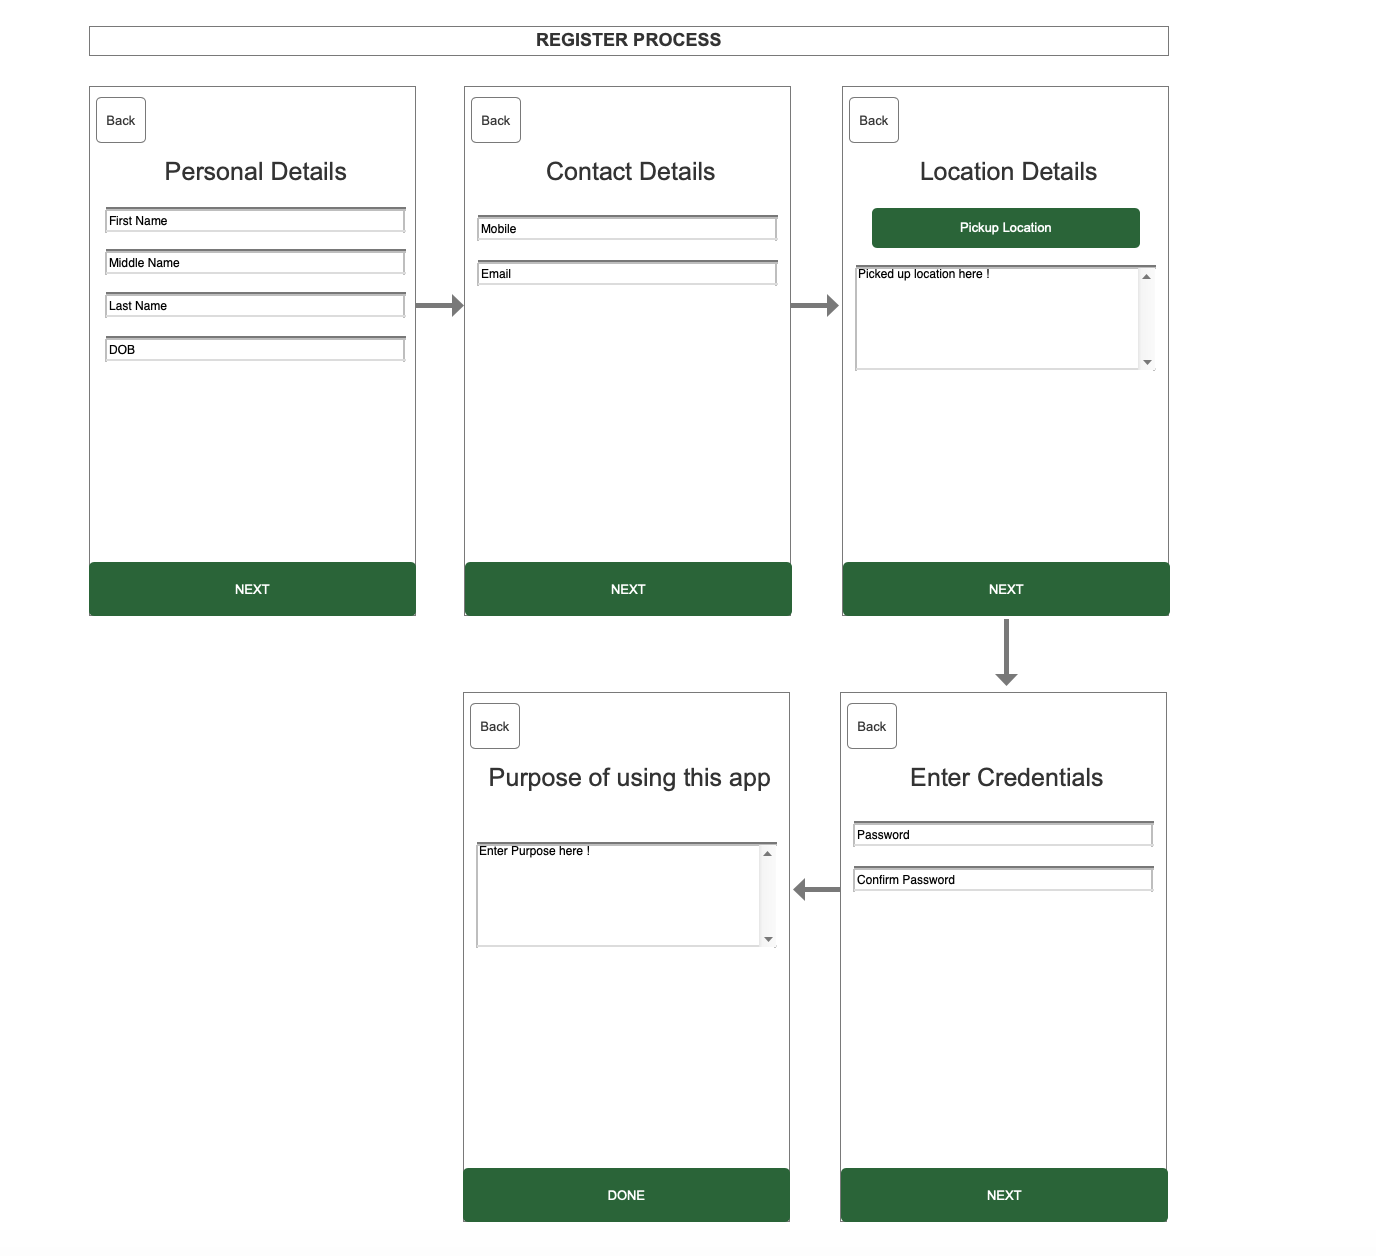
\includegraphics[width=0.5\linewidth]{figures/ch3/wireframe_1.png}
            \caption{\label{fig:wireframe_1} Wireframe - Registration process}
    \end{figure}
  
  
  
    \begin{figure}[H]
            \centering
            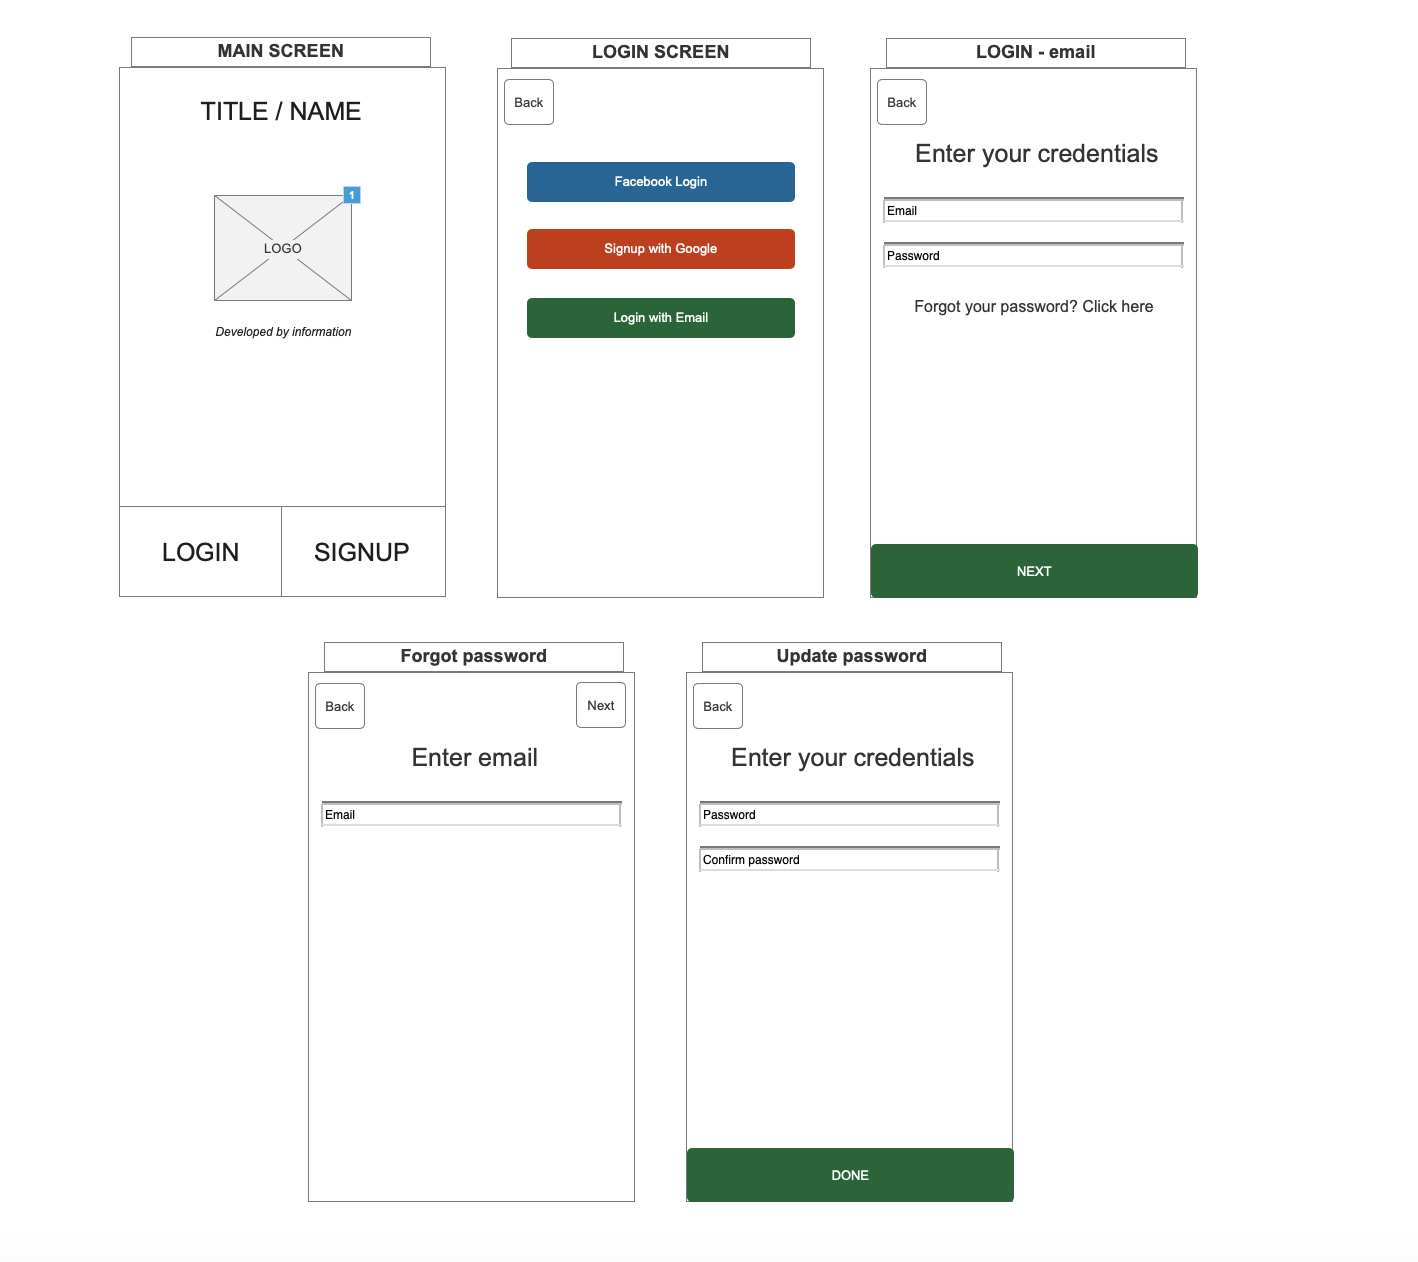
\includegraphics[width=0.5\linewidth]{figures/ch3/wireframe_2.png}
            \caption{\label{fig:wireframe_2} Wireframe - Login and forgot password process}
    \end{figure}
    
    \begin{figure}[H]
            \centering
            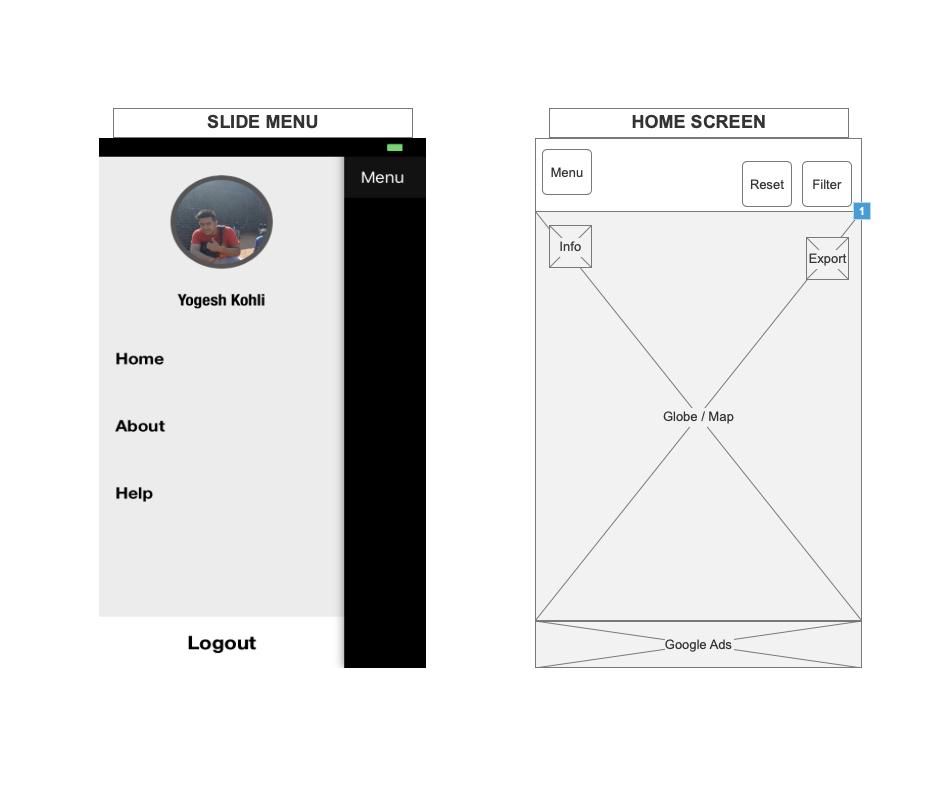
\includegraphics[width=0.5\linewidth]{figures/ch3/wireframe_3.png}
            \caption{\label{fig:wireframe_3} Wireframe - Main screen and home screen}
    \end{figure}


\section{Database Architecture}

\textbf{Definition}

An organized arrangement of information held in a \gls{pc}, particularly one that is available in different ways.


Database structure was outlined subsequent to planning \gls{uml} Diagrams in order to improve comprehension of the structure.

In the \gls{uml}, an utilization case chart can condense the subtle elements of your framework's clients (otherwise called on-screen characters) and their communications with the framework. Figure 3.8 shows the use case diagram of the app.

    \begin{figure}[H]
            \centering
            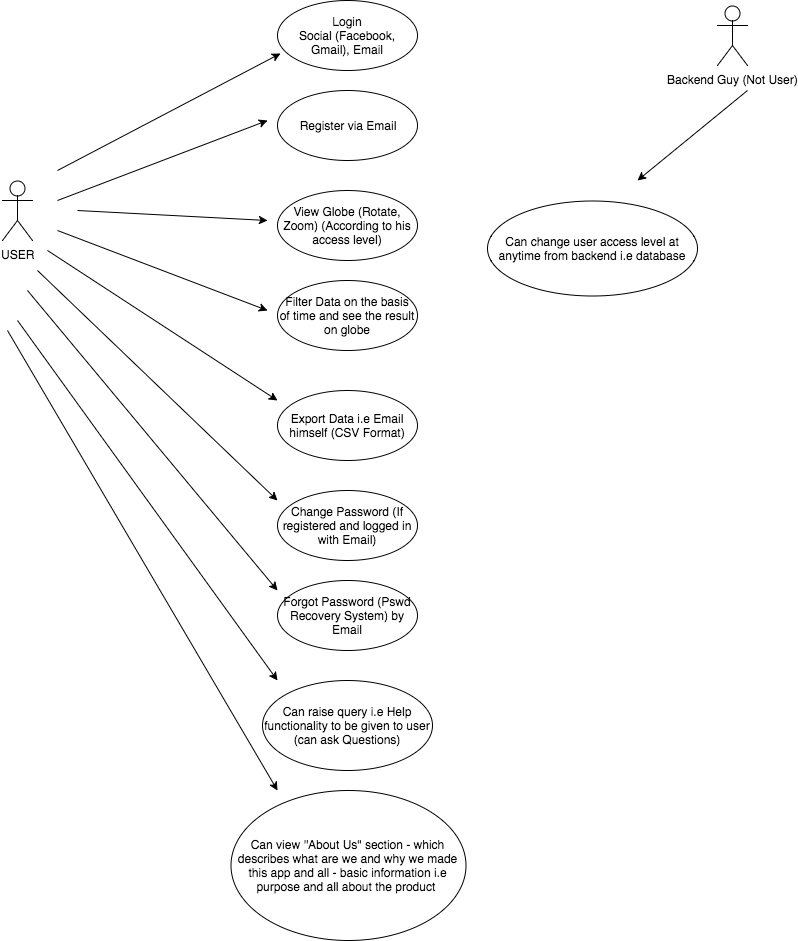
\includegraphics[width=1.0\linewidth]{figures/ch3/usecase.png}
            \caption{\label{fig:use_case} Use case diagram of the app}
    \end{figure}

As you can see in the above figure, it clearly shows the actions which user can interact with in the app.

On the other hand, Class diagrams are a standout amongst the most valuable kinds of outlines in \gls{uml} as they plainly delineate the structure of a specific framework by demonstrating its classes, characteristics, activities, and connections between articles. With our  \gls{uml} graphing programming, making these charts isn't as overpowering as it may show up. This guide will demonstrate to you generally accepted methods to comprehend, plan, and make your own class outlines. Figure 3.9 will give you better understanding how class diagrams can be used to make the product better.

    \begin{figure}[H]
            \centering
            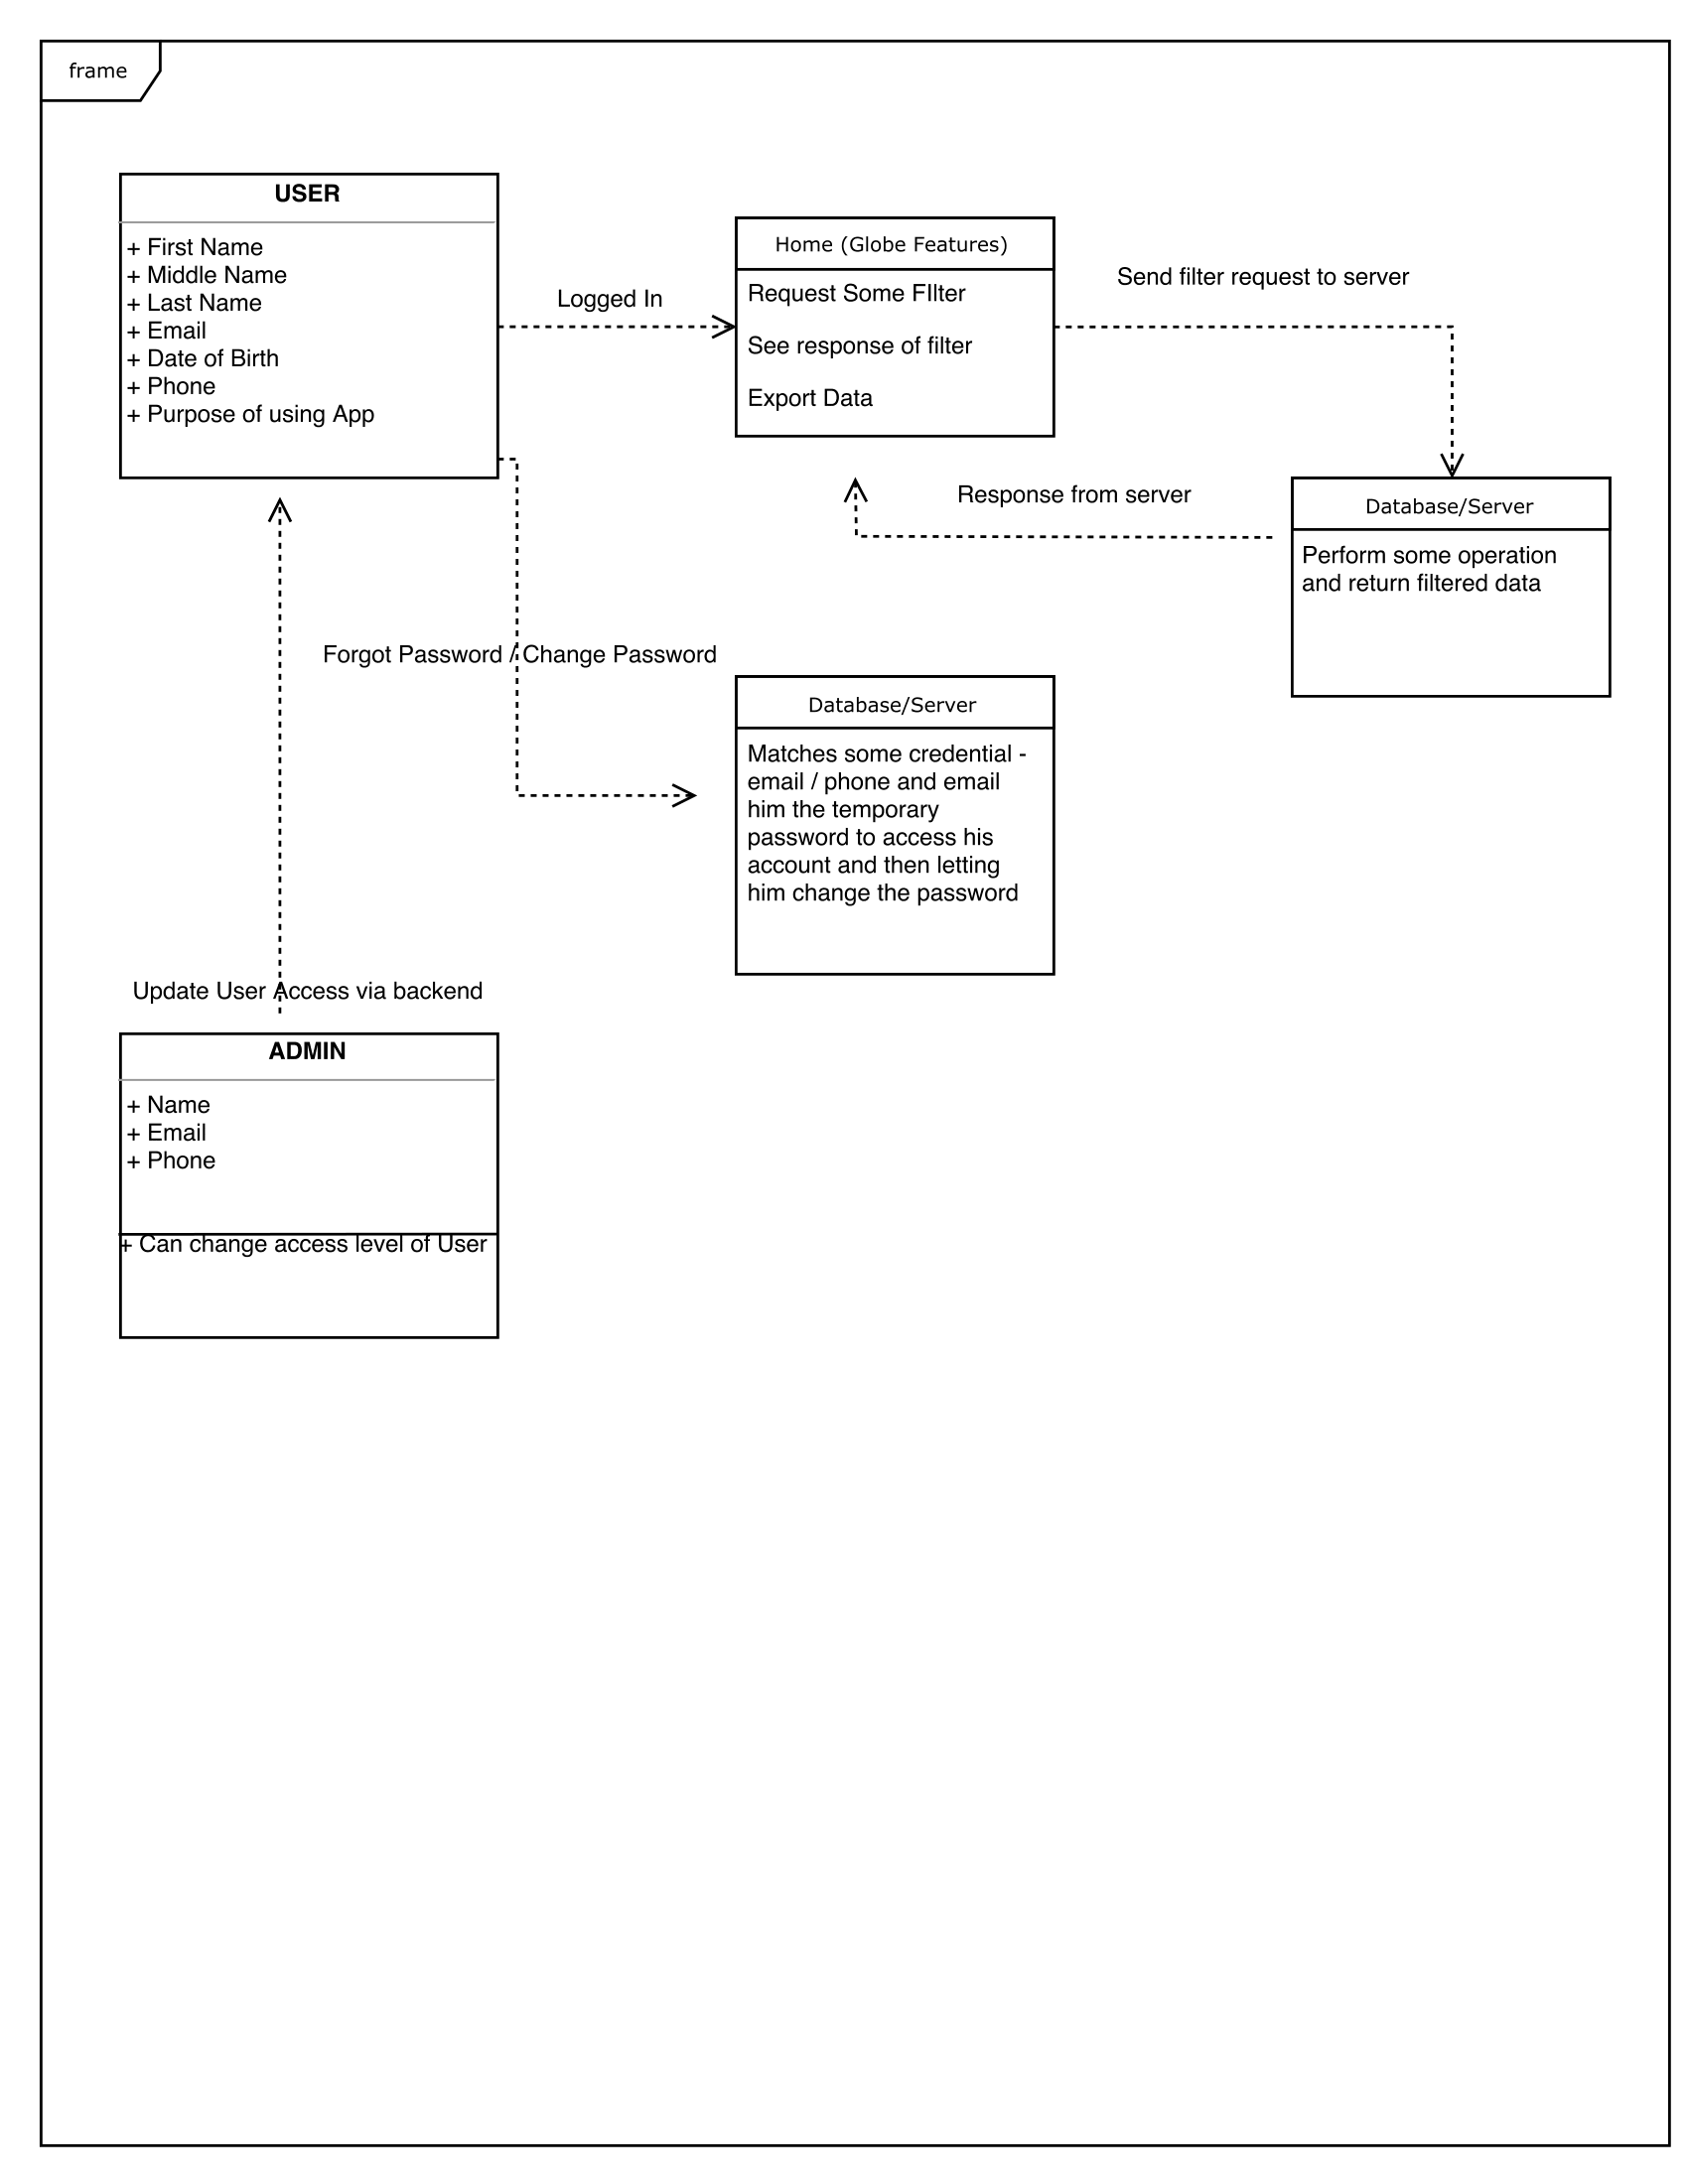
\includegraphics[width=0.8\linewidth]{figures/ch3/classdiagram.png}
            \caption{\label{fig:class_diag} Class diagram of the app}
    \end{figure}
    
    \newpage

 \centerline{\textbf{Database Structure}}    
  PostgreSQL database has been used for the project, which is a general purpose and object-relational database management system. 
  Database tables and their entities are shown in the figure 3.10.
  
  \begin{figure}[H]
            \centering
            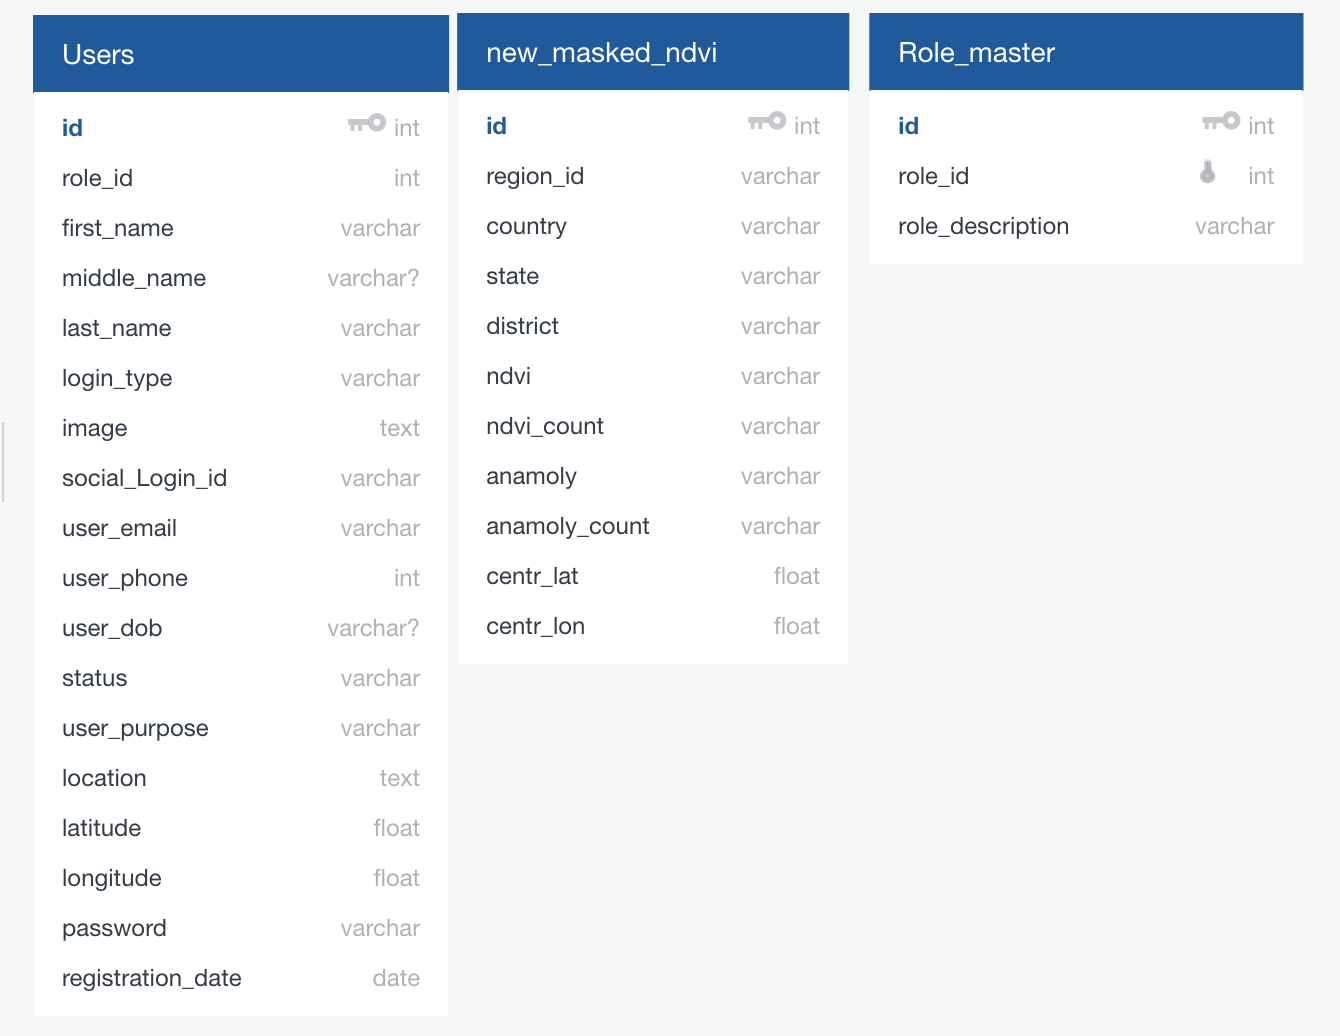
\includegraphics[width=1.0\linewidth]{figures/ch3/database_structure.png}
            \caption{\label{fig:database_structure} Database tables}
    \end{figure}
    
    




